\documentclass[11pt,a4paper,oneside]{article}
\usepackage[margin=15mm]{geometry}
\usepackage[hidelinks]{hyperref}
\usepackage{xcolor}
\usepackage{graphics}
\usepackage{tikz}
\usepackage{parskip}

\renewcommand{\familydefault}{\sfdefault}
\newcommand{\https}[1]{\href{https://#1}{\nolinkurl{#1}}}
\newcommand{\mailto}[1]{\href{mailto://#1}{\nolinkurl{#1}}}
\newcommand{\follownote}[1]{--- {\footnotesize\color{violet}#1}}
\newcommand{\prog}{Programming Lang.:}
\newcommand{\os}{Operating System:}
\newcommand{\vcs}{Version Controls:}
\newcommand{\issue}{Issue Tracking:}
\newcommand{\acmicpcnote}[2]{--- {\footnotesize\color{violet}%
\href{https://icpc.baylor.edu/regionals/finder/#1/standings}%
{#2}%
}}
\newcommand{\codejamnote}[2]{--- {\footnotesize\color{violet}%
\href{https://codingcompetitions.withgoogle.com/codejam/round/#1}%
{#2}%
}}
\renewcommand{\section}[1]{%
{\large\textbf{#1}}\\
\rule[9pt]{18cm}{.4pt}\vspace{-16pt}%
}
\newenvironment{mytable}{%
\begin{tabular}{@{}l@{\hspace{4mm}}l@{}}%
}{\end{tabular}}
\newcommand{\myitem}[2]{%
\parbox[t]{16mm}{#1}&\parbox[t]{16cm}{#2}\\%
}
\newenvironment{innertable}{%
\begin{tabular}{@{}l@{\hspace{5mm}}l@{}}%
}{\end{tabular}}
\newcommand{\inneritem}[2]{%
\parbox{35mm}{{\color{darkgray}#1}}&\parbox{12cm}{#2}\\%
}

\pagestyle{empty}

\begin{document}%
\begin{tikzpicture}[baseline=-9pt]%
\clip circle (2cm);%
\node[anchor=center] {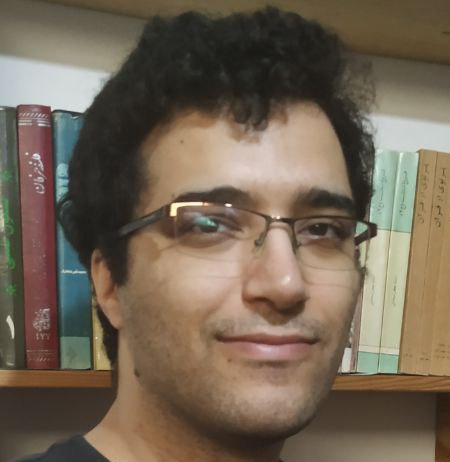
\includegraphics[width=4cm]{me}};%
\end{tikzpicture}%
\hspace{1cm}%
\parbox{13cm}{%
\begin{tabbing}%
\hspace{3cm}\=\kill%
\textbf{{\LARGE Ali Farzanrad}}\\[5mm]
Birthdate: \>
May 10\textsuperscript{th}, 1990\\[1mm]
E-Mail: \>
\mailto{ali_farzanrad@riseup.net}\\[1mm]
GitHub: \>
\https{github.com/fmwviormv}\\[1mm]
LinkedIn: \>
\https{linkedin.com/in/ali-farzanrad-0635959b}\\[1mm]
Phone: \>
+98{ }911{ }871{ }3396\\
\end{tabbing}%
}

\vspace{-9pt}%
Senior developer (\textit{high-level and low-level}) and strong
problem solver (\textit{proven in international competitions}).

\section{Professional Experience}

\begin{mytable}
\myitem{2020-04 -- current}{%
\textbf{Python Developer} at
Mahsan co., Tehran, Iran.

Developing command-line interface for company's products,
specially for firewall management.
Command-line is responsible for interacting with user through
system serial console and remote ssh pty session.
User commands varies from system configuration and diagnostic
to network utilities with support for auto-completion and
smart error handling (with nice user understandable messages).

\begin{innertable}
\inneritem{\prog}{Python 3, and Shell script}
\inneritem{\os}{Ubuntu}
\inneritem{\vcs}{Git}
\inneritem{\issue}{Gitlab}
\end{innertable}
}
\end{mytable}

\begin{mytable}
\myitem{2019-02 -- 2020-03}{%
\textbf{Developer} at
JAM Persia co., Tehran, Iran.

Developing product-planning algorithm for company's ERP system.
The algorithm is responsible for finding best selection and
schedule of resources to produce required products in time.

\begin{innertable}
\inneritem{\prog}{C\#}
\inneritem{\os}{Windows}
\inneritem{\vcs}{SVN}
\inneritem{\issue}{Jira}
\end{innertable}
}
\end{mytable}

\begin{mytable}
\myitem{2017-01 -- 2018-06}{
\textbf{Developer} at
Maharan International co., Tehran, Iran.

Developing Train Control System based on ERTMS specifications.
We were developing core functionalities for processing and
sending high-level signals.

\begin{innertable}
\inneritem{\prog}{C with Frama-C}
\inneritem{\os}{Windows}
\inneritem{\vcs}{TFS}
\inneritem{\issue}{Microsoft Project}
\end{innertable}
}
\end{mytable}

\begin{mytable}
\myitem{2012-08 -- 2016-06}{
\textbf{Developer} at
Negasht co., Tehran, Iran.

Developing web-based applications with maps and POI data.

Developing web-services for generating map tiles.

Developing web-services for generating static maps from vectors.

Developing web-services for finding shortest path by giving a
simple pair of latitude and longitudes.

Developing an Android app with so many different survey forms.

\begin{innertable}
\inneritem{\prog}{C\#, JavaScript, C++, and Java}
\inneritem{\os}{Windows}
\inneritem{\vcs}{Microsoft Visual SourceSafe}
\inneritem{\issue}{Company-specific issue tracker}
\end{innertable}
}
\end{mytable}

\section{Education}

\begin{mytable}
\myitem{2015}{
\textbf{MSc in Computer Science, Major in Intelligent Systems}

Amirkabir University of Technology (Tehran Polytechnic), Tehran, Iran
}
\end{mytable}

\pagebreak

\section{Awards and Honors}

\begin{mytable}\myitem{2017}{
Ranked 474\textsuperscript{th} among over 25{ }000 contestants
\codejamnote{0000000000201900}{Google CodeJam Round 2}
}\end{mytable}

\begin{mytable}\myitem{2015}{
Ranked 2\textsuperscript{nd} in Ph.D. enterance exam
\follownote{National University Entrance Exam}
}\end{mytable}

\begin{mytable}\myitem{2013}{
Ranked as 2\textsuperscript{nd} university among all
national universities
\acmicpcnote{Tehran-2013}{ACM-ICPC Asia Tehran Regional Contest}
}\end{mytable}

\begin{mytable}\myitem{2013}{
Ranked 67\textsuperscript{th} among over 2{ }000 universities
\follownote{The 37\textsuperscript{th} ACM-ICPC World Finals}
}\end{mytable}

\begin{mytable}\myitem{2012}{
Ranked 1\textsuperscript{st} among 66 teams
\acmicpcnote{Kanpur-2012}{ACM-ICPC Asia Kanpur Regional Contest}
}\end{mytable}

\begin{mytable}\myitem{2012}{
Ranked 6\textsuperscript{th} in M.Sc. enterance exam
\follownote{National University Entrance Exam}
}\end{mytable}

\begin{mytable}\myitem{2011}{
Ranked 4\textsuperscript{th} among 76 teams
\acmicpcnote{Tehran-2011}{ACM-ICPC Asia Tehran Regional Contest}
}\end{mytable}

\begin{mytable}\myitem{2007}{
Rewarded as Silver in National Olympiad in Informatics
}\end{mytable}

\section{Programming Languages}
\begin{itemize}
\item C (C89/90, C99, C11, libevent, pthreads, yacc, lex)
\item Python (Python 3.x, async)
\item C++ (C++98, C++11, C++14)
\item Java (Java 7, Java 8)
\item C\# (.Net Framework 4.x, ASP.NET MVC, .Net Core 2.x \& 3.x)
\item JavaScript (ES5.x, ES6)
\item Assembly (6502, 8086, i386, amd64, intel/at\&t syntax, SIMD)
\item UNIX Shell (sh, ksh, bash, sed, awk)
\end{itemize}

\section{Languages}

\begin{mytable}\myitem{Persian}{
	Native
}\end{mytable}

\begin{mytable}\myitem{English}{
	B2, TOEFL 79
}\end{mytable}

\begin{mytable}\myitem{German}{
	A1
}\end{mytable}

\end{document}
